
\begin{figure}[bt]
\centerline{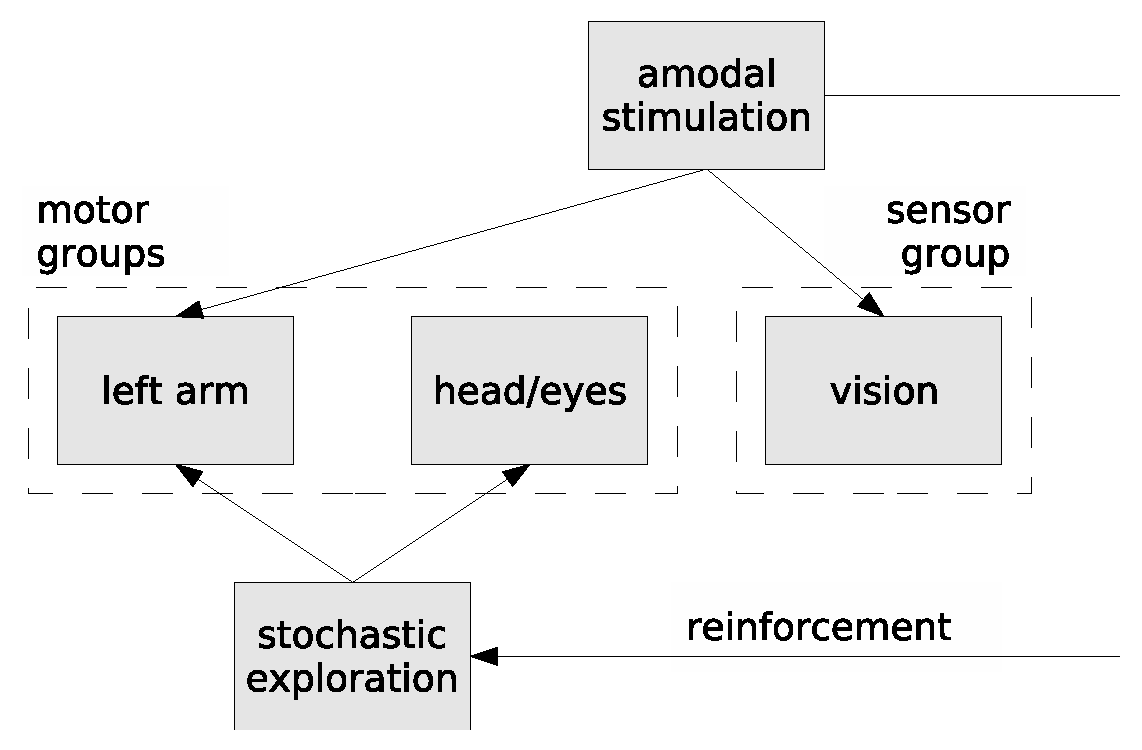
\includegraphics[height=6cm]{images/amodal-modules}}
\caption {
%
\label{fig:amodal-module-vision}
%
The system for stochastic exploration and amodal stimulation.
Exploration exercises a set of motor groups, moving them
to random locations within their nominal ranges.
Amodal stimulation modulates the state of a motor group
in a rhythmic fashion, and looks for signs of that rhythm 
showing up in a sensor group. If the amodal signal does in
fact get transmitted, a reinforcement signal is sent to the
exploration model, biasing further exploration towards the
current configuration of the motor groups.
%
The specific scenario shown here is for visual hand/arm coordination.
The state of the head and arm are explored, while watching for
an amodal connection between the arm and vision.
%
}
\end{figure}

\section{Stochastic exploration and amodal stimulation}

\label{sect:motor-babble}



In \citeasnoun{fitzpatrick2007shared}, we identified three basic scenarios in
which a robot's body can be recruited in solving perceptual tasks:

\liststyleLiii
\begin{enumerate}
\item \textstyleEmphasis{direct exploration}: the body in this case is
the interface to extract information about the objects. For example in
\citep{natale04learning} haptic information was employed to distinguish objects
with different shapes, a task that would be much more difficult if
performed visually. In
\citep{torres-jara05tapping} the robot learned to recognize a few objects by using
the sound they generate upon contact with the fingers. 
\item \textstyleEmphasis{controlled exploration}: use the body to
perform actions to simplify perception. The robot can deliberately
generate redundant information by performing periodic actions in the
environment. The robot can also initiate actions and wait for the
appearance of consequences
\citep{fitzpatrick03grounding}. 
\item \textstyleEmphasis{the body as a reference frame}: during action
the hand is the place where important events are most likely to occur.
The ability to direct the attention of the robot towards the hand is
particularly helpful during learning; in
\citep{natale05exploring} we show how this ability allows the robot to learn a
visual model of the objects it manages to grasp by simply inspecting
the hand when touch is detected on the palm. 
%
In similar situations the same behavior could allow the robot to
direct the gaze to the hand if something unexpected touches
it. Eye-hand coordination seems thus important to establish a link
between different sensory channels like touch and vision.
\end{enumerate}



As part of the CONTACT project, we have been experimented with scenario (2),
controlling exploration.  In particular, we are looking for mechanisms for
learning that are applicable to both speech and
manipulation.
%
This work revisits themes already examined in prior work, but under a
more general framework.

Figure~\ref{fig:amodal-module-vision} shows a crude but general system
for learning motor-sensor mappings, applied to the problem of hand-eye
coordination for concreteness.  We assume that the learning problem
can be posed as follows: given a collection of motor groups and sensor
groups, and a particular feature derived from the sensed data, the
task is to find a configuration of the motor groups such that local
changes in that configuration lead to systematic changes in the
derived feature.  This would correspond, for example, to moving 
a head and arm such that the one is looking at the other, as opposed to
the arm being out of view behind the body or off to the side.

More formally, suppose we have motor control variables
$m=(m_1,m_2,...,m_N)$ and sensor variables $s=(s_1,s_2,...,s_n)$.
Suppose we have some chosen feature of interest $f(s)$.  We know that
$s$ is a function of both $m$ and a set of environmental variables
representing all other influences and state, $e=(e_1,e_2,...)$.
We are interested in how $f$ changes with $m$:

\begin{equation}
\nabla f  = \left(\frac{\partial f}{\partial m_1 }, \frac{\partial f}{\partial m_2 }, \dots,  \frac{\partial f}{\partial m_N }  \right)
\end{equation}

We would like to maximize $|\nabla{}f|$.  We estimate this value
directly through measurement by systematically perturbing $m$ and
measuring $f$.
%
In fact, we really are only concerned with making $|\nabla{}f|$ 
non-zero, since it is quite possible that in much of the motor space 
changes in $m$ have completely no impact on $f$.
%
In that case, we can measure the change in a random motor 
direction $\Delta{}m=(\Delta{}m_1,\Delta{}m_2,...,\Delta{}m_N)$.
%
Unless we are unlucky enough to pick a direction orthogonal to 
the gradient, we should see some change in $f$.
%
However, as we are perturbing $m$, other environmental variables
may also have been changing, causing arbitrary effects on $f$.
We can make this less problematic by simply repeating our perturbation
rhythmically and seeing if the behavior on $f$ seems truly
systematic.

When we detect that $f$ appears to be influenced by $m$ in this
sense, we have discovered a configuration of $m$ which could
be useful as a starting point for exploring the local mapping
from motors ($m$) to sensors ($s$) or between sets of motors.
We call this a ``resonance.''
In the abstract, this event is similar to the 
infant's ``discovery'' of its hand in its field of view.
Figures~\ref{fig:amodal-module-vision} and \ref{fig:find-arm}
show an analogous experiment for a robot, where a configuration
of the arm and head
is discovered that brings the arm into view.

Since $f$ is computed based on sensor input, we should
expect to occasionally be misled.  Therefore, rather 
than stopping once we find a good value of $m$, we use
a stochastic search method.  
%
Currently, we maintain a population of possible motor configurations,
initially random.  In each step, we select a configuration randomly,
perturb it (or with a small probability randomize it entirely), and if
it results in an apparent resonance, we copy that configuration to 10\%
of the population.
%
A configuration that consistently results in resonance therefore quickly 
propagates to the entire population.
%
This is the evolution being shown in Figure~\ref{fig:find-arm}.

\begin{figure}[p]
\centerline{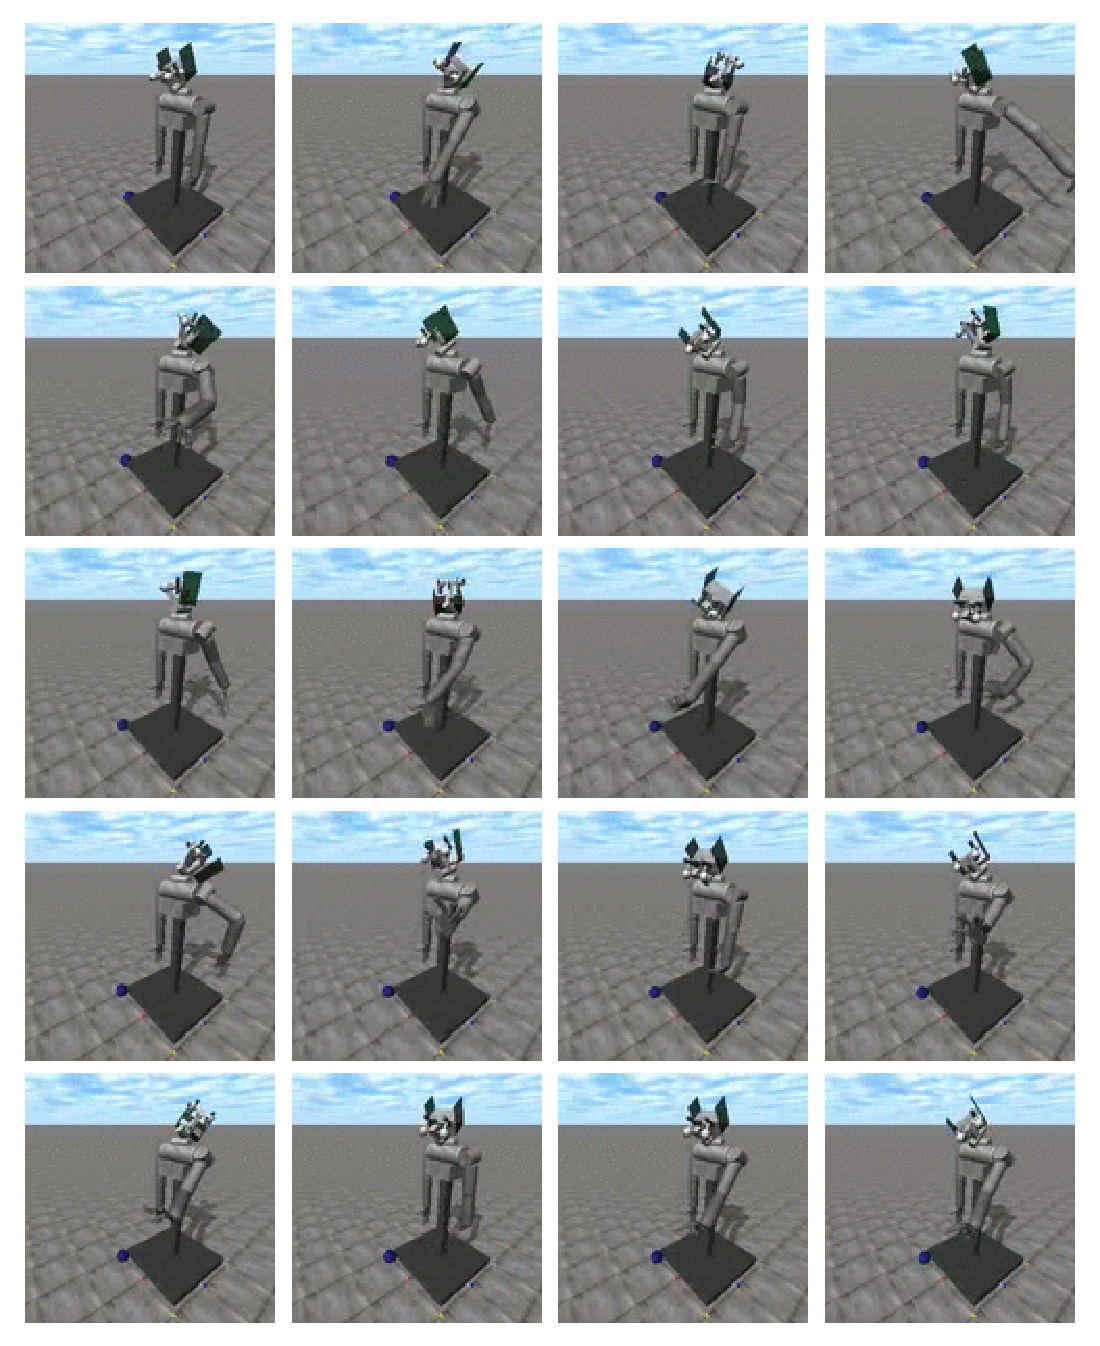
\includegraphics[width=\textwidth]{images/find-arm}}
\caption{
%
\label{fig:find-arm}
%
A simulated robot, performing motor exploration on its
head/eyes and left arm.  The head, eyes, and arms move around randomly
within their range of movement.
%
A periodic ``shaking'' movement of the arm is made about its
current position, and the effect of this movement is searched 
for visually.
%
When resonance occurs, the configuration of head/eyes and left arm
is reinforced so that the robot is more likely to return to that
configuration.
%
This is why 
in early snapshots (top) the robot is unlikely to be looking at 
its arm, and in later snapshots (bottom) the robot is looking at
its arm more often than not.
%
}
\end{figure}


We would like to stress that developing a general purpose learning
mechanism of this kind for a robot does not mean we believe the robot
should start off its developmental process as a ``tabula rasa.''  In
fact, there may well be just as much or more information involved in
specifying how to explore (expressing the motor groups to use, their
scales, and what sensory cue to monitor) as there would be in just
giving numerical pose information.
%
The advantage we are looking for is robustness to the details of 
the motor and perceptual system, such that changes in scale or the
ranges of joints do not disrupt everything.
%
We want a way of expressing capabilities such as ``bring the hand in
front of head'' which can be developed operationally, rather than
relying on parameters supplied for a particular instantiation
of a robot body.

As a side benefit, our robot should not be completely stumped if
expected to control its arm as seen via a mirror or other distortion.
Any transformation that is spatially smooth should be manageable;
however delays introduced in perception would be as disastrous for our
system as they are for humans.

Of course, the specific method described so far is very crude.  It is
intended only to locate an initial point of contact between motor
spaces or between motor and sensor spaces.  Once that point has been
found, tracking methods would be more efficient for exploring a region
of motor space.



%%Could automate motor space classification examples: gesture
%%recognition, speech recognition

%%Would have to be a lot simpler than offline, human-mediated work of course.


%% \subsection{Towards meaning}

%% The richer the robot's "internal life" is, the more interesting kinds
%% of "meanings" there can be in its world

%% - Continuous, broad, shared, structured experience

%% - Meaning as a process, not a label

%% Off-line data collection, segmentation, labelling, training of
%% classifiers, etc work, but restrict the potential semantic universe of
%% the robot.

%% For Year 3, online behaviors would be useful.


